\chapter[Metodolodia]{Metodologia}

Para investigar a prática atual de avaliação de desenvolvedores, é preciso olhar mais profundamente em como as empresas o fazem. No propósito de conduzir esse estudo, foi decidido executar uma pesquisa com sujeitos humanos para extrair a informação desejada e analisá-la. Neste estudo foi pedido para os respondentes primeiro classificar o desenvolvedor (em níveis de importância), e depois preencher o resto do formulário com as características do desenvolvedor.

Para analisar os dados obtidos, serão utilizados métodos de classificação para se obter uma visão clara em como as características afetam a classificação dos supervisores, e como produto, dependendo dos dados encontrados, obter um classificador que possa ser utilizado para ajudar os supervisores a ganhar \textit{insights} de como melhorar a importância geral do time.

Esta seção se dedica a explicar o desenho desse experimento, mostrando a criação e a aplicação da pesquisa com os supervisores, e mostrar também como foi conduzida a análise dos dados obtidos dessa pesquisa, incluindo a análise de critérios e a construção do classificador.

\section{Pesquisa}\label{secao3.2}

Nas próximas subseções serão tratadas a abordagem utilizada para compor a pesquisa, a aplicação da pesquisa em si nos supervisores das empresas participantes e a caracterização dos mesmos.

\subsection{Goal-Question-Metric}\label{secao3.2.1}
Foi utilizada uma abordagem chamada Goal-Question-Metric(GQM) \cite{Basili1994} que ajudou a compor a pesquisa. GQM é uma abordagem do tipo top-down, que é baseada no pressuposto que primeiro, para se medir algo, é necessário especificar objetivos (goal), dos quais é possível derivar perguntas (question), e então, especificar as métricas (metric) que precisam ser coletadas para responder essas perguntas.

Para atingir o propósito de um objetivo, é necessário determinar 3 coordenadas:

\begin{alineas}
	\item \textbf{Questão \textit{(issue)}:} Qual questão/assunto está sendo lidado;
	\item \textbf{Objeto/Processo \textit{(object/process)}:} Qual é o objeto central da análise;
	\item \textbf{Ponto de vista \textit{(ViewPoint)}:} Sob a perspectiva de quem a análise está sendo feita.
\end{alineas}
	
A \autoref{tabela2} mostra o modelo GQM, com o propósito, as perguntas derivadas do mesmo e as métricas levantadas para responder essas perguntas.


\begin{table}[h]
	\footnotesize
	\caption{Goal-Question-Metric}
	\label{tabela2}
	\def\arraystretch{1.5}
	\begin{tabular}{|p{2cm}|p{6.25cm}|p{6.25cm}|}
		\hline
		\multirow{4}{*}{\textbf{Objetivo}} & \textbf{Propósito}                              & Medir                                                 \\ \cline{2-3} 
		& \textbf{Questão}                                & a importância                                         \\ \cline{2-3} 
		& \textbf{Objeto}                                 & do desenvolvedor                                      \\ \cline{2-3} 
		& \textbf{Ponto de vista}                         & sob a perspectiva do supervisor                       \\ \hline
		\textbf{Pergunta}                  & \multicolumn{2}{l|}{Qual a produtividade desse desenvolvedor?}                                          \\ \hline\hline
		\multirow{2}{*}{\textbf{Métricas}} & \multicolumn{2}{l|}{Quantidade de entregas por mês}                                                     \\ \cline{2-3} 
		& \multicolumn{2}{l|}{Avaliação subjetiva da produtividade}                                               \\ \hline\hline
		\textbf{Pergunta}                  & \multicolumn{2}{l|}{\parbox{12cm}{ Qual o nível de habilidade técnica que o desenvolvedor em questão possui?}}          \\ \hline
		\multirow{4}{*}{\textbf{Métricas}} & \multicolumn{2}{l|}{Experiência relevante}                                                              \\ \cline{2-3} 
		& \multicolumn{2}{l|}{Conhecimento especializado}                                                         \\ \cline{2-3} 
		& \multicolumn{2}{l|}{Diversidade de habilidades}                                                         \\ \cline{2-3} 
		& \multicolumn{2}{l|}{Resolução de problemas complexos}                                                   \\ \hline\hline
		\textbf{Pergunta}                  & \multicolumn{2}{l|}{\parbox{12cm}{Qual o nível de habilidade interpessoal que o desenvolvedor em questão possui?}}     \\ \hline
		\multirow{2}{*}{\textbf{Métricas}} & \multicolumn{2}{l|}{Comunicação com colegas}                                                            \\ \cline{2-3} 
		& \multicolumn{2}{l|}{Disposição para ajudar colegas quando solicitado}                                   \\ \hline\hline
		\textbf{Pergunta}                  & \multicolumn{2}{l|}{\parbox[c][1cm][c]{12cm}{Quando se depara com um problema, qual o principal comportamento do desenvolvedor?}} \\ \hline
		\multirow{4}{*}{\textbf{Métricas}} & \multicolumn{2}{l|}{(Introspectivo) Tenta resolver sozinho}                                             \\ \cline{2-3} 
		& \multicolumn{2}{l|}{(Introspectivo) Busca na documentação e livros}                                     \\ \cline{2-3} 
		& \multicolumn{2}{l|}{(Comunicativo) Procura ou pergunta em sites de perguntas e respostas}               \\ \cline{2-3} 
		& \multicolumn{2}{l|}{(Comunicativo) Pede ajuda para os colegas ou supervisores}                          \\ \hline\hline
		\textbf{Pergunta}                  & \multicolumn{2}{l|}{\parbox{12cm}{Qual o nível dessas características no perfil comportamental do desenvolvedor?}}     \\ \hline
		\multirow{4}{*}{\textbf{Métricas}} & \multicolumn{2}{l|}{Liderança}                                                                          \\ \cline{2-3} 
		& \multicolumn{2}{l|}{Criatividade}                                                                       \\ \cline{2-3} 
		& \multicolumn{2}{l|}{Empreendedorismo}                                                                   \\ \cline{2-3} 
		& \multicolumn{2}{l|}{Pró-atividade}                                                                      \\ \hline\hline
		\textbf{Pergunta}                  & \multicolumn{2}{l|}{\parbox{12cm}{Qual o compromisso do desenvolvedor em relação à empresa?}}                          \\ \hline
		\multirow{4}{*}{\textbf{Métricas}} & \multicolumn{2}{l|}{Tempo de trabalho}                                                                  \\ \cline{2-3} 
		& \multicolumn{2}{l|}{Organização e planejamento}                                                         \\ \cline{2-3} 
		& \multicolumn{2}{l|}{Foco no cliente}                                                                    \\ \cline{2-3} 
		& \multicolumn{2}{l|}{Foco nos resultados}                                                                \\ \hline
	\end{tabular}
\end{table}

\subsection{Aplicação da Pesquisa}

A pesquisa foi aplicada de maneira remota, para dar a liberdade necessária para os respondentes participarem da pesquisa. Para isso, foi utilizada a ferramenta de formulários do Google (Google Form).

Para preservar a privacidade das empresas participantes, não foi solicitado nenhum tipo de identificação, tanto do respondente como do desenvolvedor sendo analisado. A única identificação solicitada foi o nome da empresa de onde vinham as avaliações. Foi necessário solicitar esse dado para uma investigação mais profunda nos casos em que as empresas atingiam o mínimo de 10 desenvolvedores avaliados.

\subsection{Caracterização dos respondentes}\label{caracterizacao_respondentes}

A pesquisa foi projetada para ser aplicada em empresas que possuem uma área de desenvolvimento de software, com uma estrutura hierárquica mínima onde existisse o cargo de supervisor, ou gerente, ou engenheiros-chefe, etc (para futuras referências, essa pessoa será referenciada como supervisor).

Os respondentes da pesquisa são então supervisores de times de desenvolvimento. Entende-se que eles são as pessoas certas para o fazer, porque diferentemente do dono da empresa eles estão perto o suficiente do dia a dia de trabalho, e conseguem julgar quais os desenvolvedores mais importantes, mesmo que eles não usem um método formalizado para tal. Eles devem responder a avaliação para cada desenvolvedor.

\section{Seleção de Características}\label{secao3.3}

No intuito de conduzir a análise dos critérios para determinar quais fatores são os mais relevantes e possuem maior influência na avaliação do supervisor, foi utilizada a ferramenta WEKA\cite{Holmes}.

Vários problemas reais possuem diversas características envolvidas (mostradas na \autoref{tabela2}), e apenas algumas dentre elas são relevantes para o objetivo final \cite{Kira1992}, neste caso, classificar a importância de um desenvolvedor. Para resolver esse problema, será utilizada uma estratégia chamada seleção de características (do inglês, Feature Selection), onde será selecionado um subconjunto de características para se ter em foco, e ignorar o restante para acelerar o processo de aprendizado, aprimorar a qualidade do classificador e atingir a melhor acurácia do algoritmo de aprendizado de máquinas \cite{Kira1992,Kohavi1997}. 

O algoritmo que será utilizado é chamado GainRatioAttributeEval, que avalia os atributos um a um independentemente e os ordena de acordo com sua influência sobre a classe. A seleção de características escolhe baseada nessa ordenação, e isso permite eliminar atributos irrelevantes. Esse método, como não avalia um subconjunto de atributos, não elimina atributos redundantes (apenas os irrelevantes), mas isso não é um problema, pois todos os atributos são conhecidos e esse tipo de avaliador não necessita de um método de busca, o que o torna muito rápido em sua execução.

\section{Classificação}\label{secao3.4}

Como resultado dessa pesquisa, será gerado um conjunto com várias avaliações de supervisores sobre os desenvolvedores. Nesse conjunto serão aplicados algoritmos de aprendizado de máquinas, no intuito de gerar um classificador de importância. Os algoritmos de aprendizado de máquinas precisam de dois conjuntos de dados: um para realizar o treinamento e um para testar o resultado, para verificar a acurácia do classificador. A \autoref{fig_1} mostra o processo que melhor representa esse cenário.

\begin{figure}[h]
	\centering
	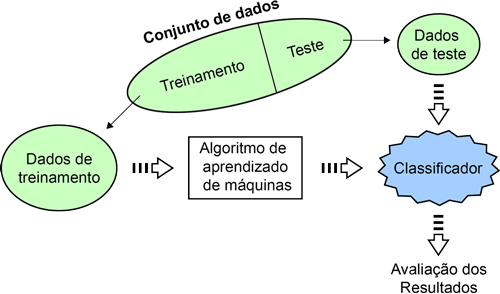
\includegraphics[scale=0.7]{figs/training-datasets-pequeno.png}
	\caption{\label{fig_1}Processo dos algoritmos de aprendizado de máquinas}
\end{figure}

Existe uma variedade de métodos para avaliar a performance de um classificador. É possível, por exemplo, selecionar uma porcentagem de um conjunto de dados para aplicar os algoritmos de aprendizado de máquinas e usar o resto para teste. O método de avaliação padrão e mais confiável é chamado cross-validation. Neste caso, será utilizado o 10-fold cross-validation que divide o conjunto em 10 partes iguais (as chamadas folds), usa 9 partes dessa divisão para treinamento e guarda uma parte para teste, e depois, faz isso mais 9 vezes, sempre alternando o pedaço utilizado para teste, assim, uma determinada parte é usada 9 vezes para treinamento e uma para teste. O resultado será a média das 10 vezes que o algoritmo executou.

Os algoritmos de aprendizado de máquina que serão utilizados são o J48, um classificador em árvore, e o NaïveBayes, um classificador bayesiano.

J48 é uma variação de um famoso sistema chamado C4.5, que foi descrito por Quinlan \cite{Quinlan1993} que usa árvores de decisão para construir um classificador (WEKA inclusive fornece uma visão da árvore gerada com todos os seus pesos.

NaïveBayes é um método probabilístico que possui duas assunções: que os atributos são igualmente importantes e estatisticamente independentes (essa assunção de independência nunca é 100\% correta, mas os métodos baseados nela geralmente funcionam bem na prática). Observando as métricas que serão coletar e o conjunto de dados que será gerado após a aplicação da pesquisa, esses dois métodos parecem servir bem aos propósitos deste estudo.

Será utilizado também um terceiro algoritmo chamado AttributeSelectClassifier, que na verdade usa um método de seleção de características (nesse caso, o GainRatio) e um algoritmo para executar a classificação (nesse caso, J48 ou NaïveBayes). Esta é uma maneira mais apropriada para aplicar seleção de características porque assim o algoritmo seleciona as características no conjunto de treinamento, tornando os resultados mais confiáveis.

Por fim, para conduzir todas essas análises será utilizado um modo do programa WEKA chamado EXPERIMENTER, que permite rodar o mesmo experimento mais de uma vez e determinar a média e o desvio padrão, para evitar falsos resultados otimistas ou pessimistas (alta ou baixa acurácia) devido à seleção de atributos nos conjuntos de treinamento e teste. Esse modo permite comparar os resultados de diferentes algoritmos.






















